\section{KDE Multimedia}

\subsection{Grabación de CDs/DVDs}
\frame
{
	\frametitle{K3b: el kreador de CDs y DVDs}
	\begin{center}
		
\includegraphics[height=6cm]{./imgs/k3b.jpg}
	\end{center}
}

\subsection{Reproducción de Video}
\frame
{
	\frametitle{Kaffeine}
	\begin{center}
		
\includegraphics[height=6cm]{./imgs/kaffeine.jpg}
	\end{center}
}

\subsection{Gestión/Reproducción de Audio}
\frame
{
	\frametitle{amaroK}
	\begin{center}
		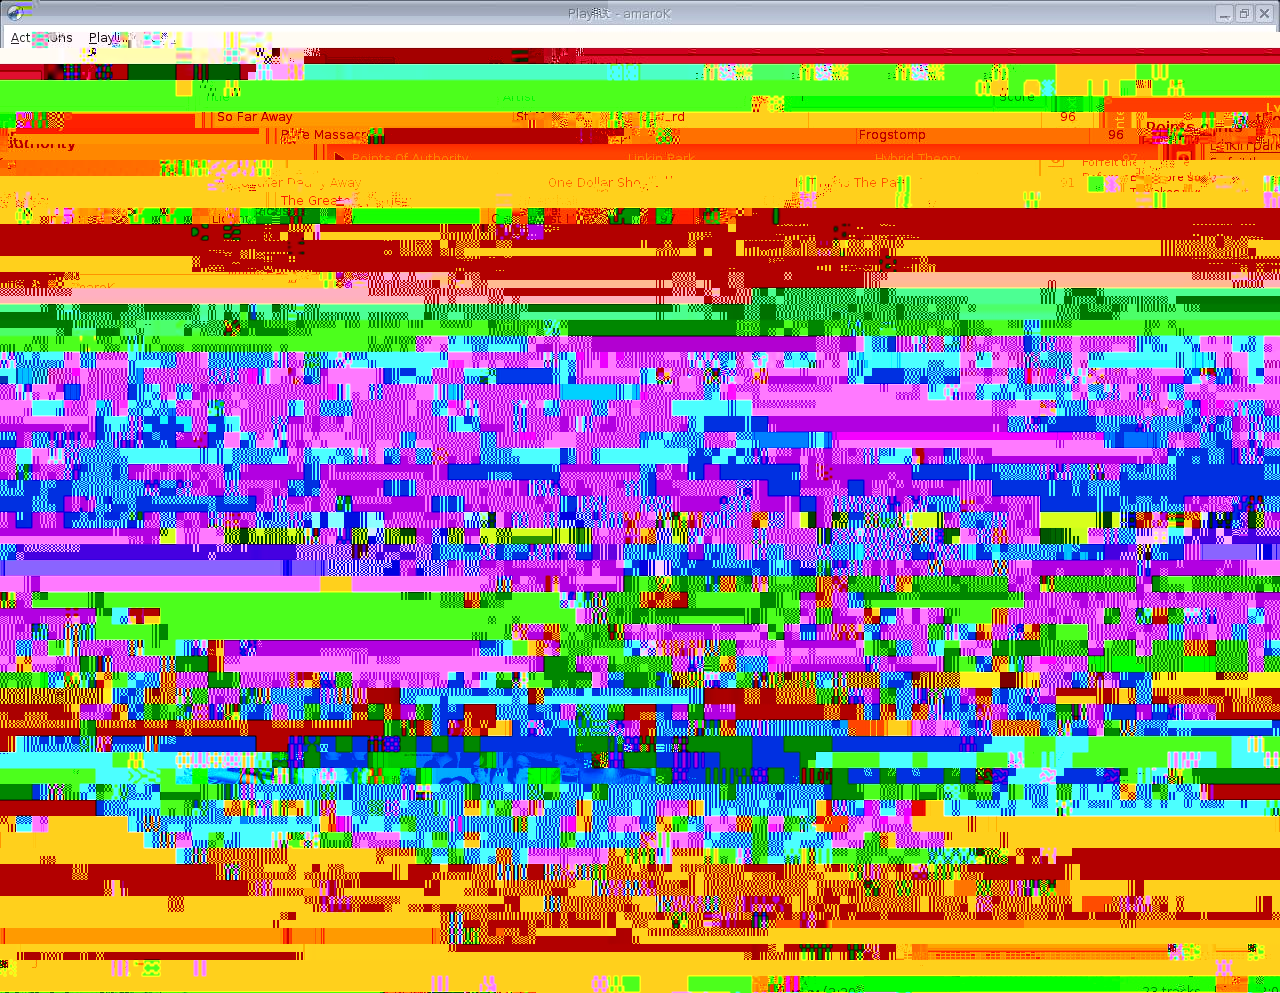
\includegraphics[height=6cm]{./imgs/amarok.jpg}
	\end{center}
}

\subsection{Edición de Video}
\frame
{
	\frametitle{Kino}
	\begin{center}
		
\includegraphics[height=6cm]{./imgs/kino.jpg}
	\end{center}
}

\subsection{Multimedia no KDE}
\frame
{
	\frametitle{Mplayer: Reproductor de Video}
	\begin{center}
		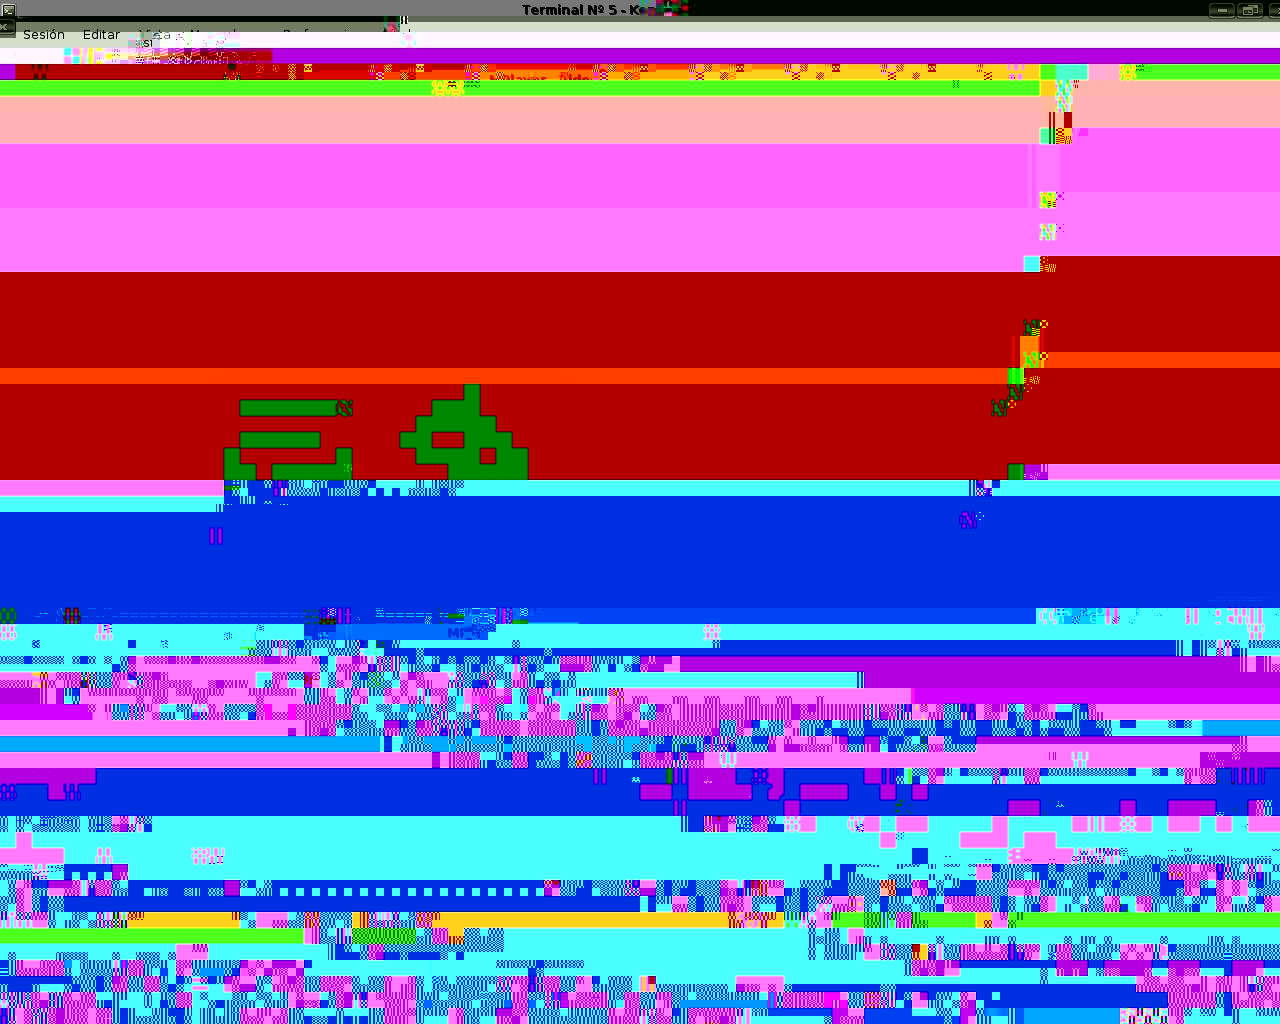
\includegraphics[height=6cm]{./imgs/mplayer.jpg}
	\end{center}
}

\frame
{
	\frametitle{Xine: Reproductor de Video}
	\begin{center}
		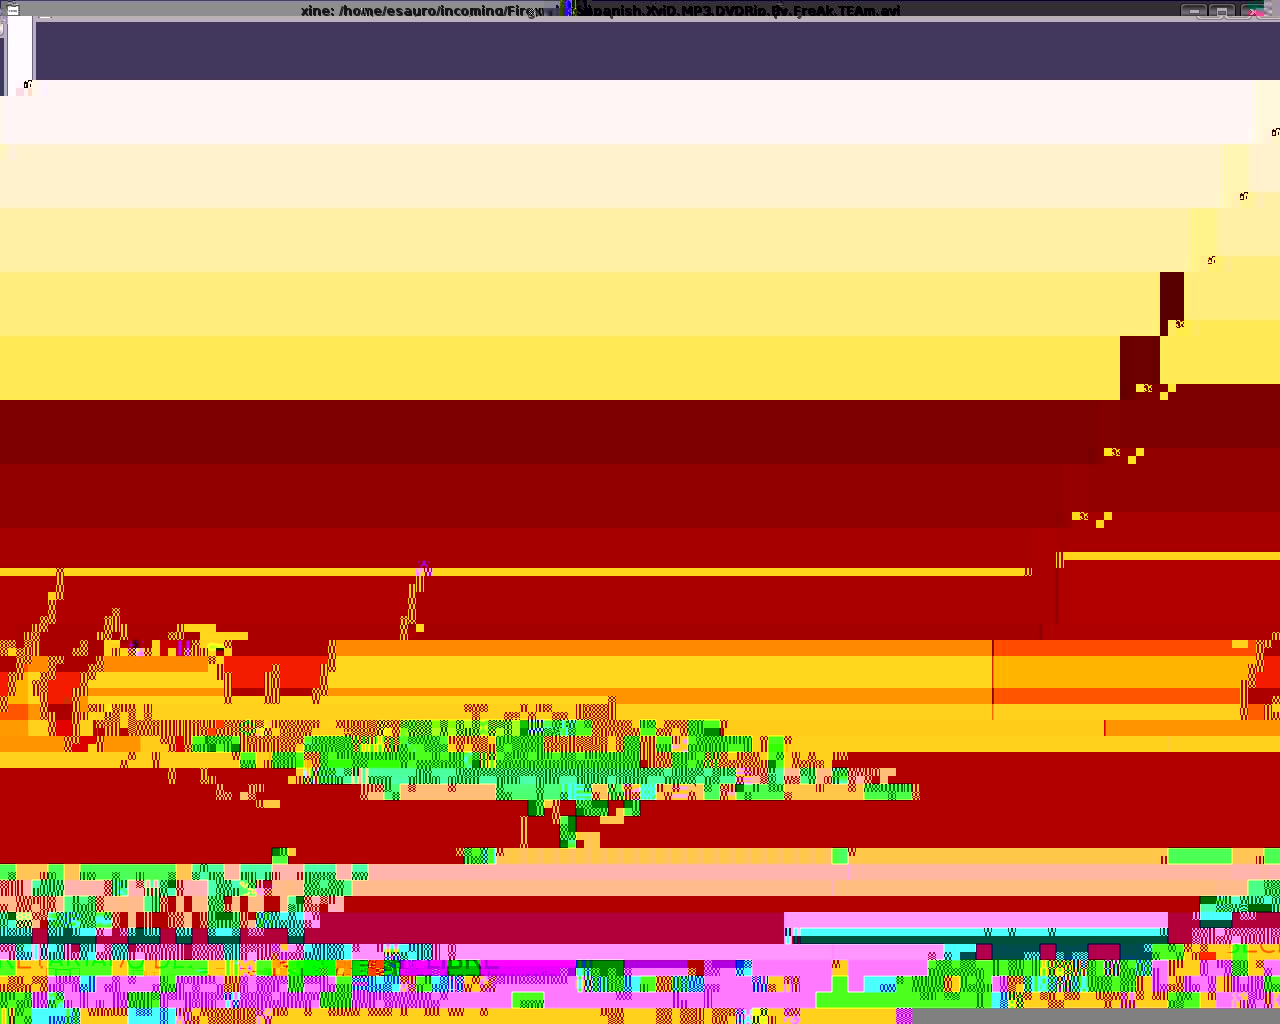
\includegraphics[height=6cm]{./imgs/xine1.jpg}
	\end{center}
}

\frame
{	
	\frametitle{XMMS: Reproductor de Audio}
	\begin{center}
		\includegraphics[height=6cm]{./imgs/xmms.jpg}
	\end{center}
}

\frame
{
	\frametitle{Audacity: Editor de Audio}
	\begin{center}
		\includegraphics[height=6cm]{./imgs/audacity-linux.png}
	\end{center}
}

